\documentclass[12pt]{article}

% ~--  Encoding & fonts (pdfLaTeX route) ~-- 
\usepackage[T1]{fontenc}
\usepackage[utf8]{inputenc}
\usepackage{lmodern}
\usepackage{microtype}
\usepackage{amsfonts}
\usepackage{tipa}

% ~--  Figures & tables ~-- 
\usepackage{graphicx}
\usepackage{array}
\usepackage{booktabs}
\graphicspath{{./}{figs/}}

% ~--  Page layout & spacing ~-- 
\usepackage{geometry}
\geometry{margin=1.25in}
\usepackage{setspace}
\doublespacing
\setlength{\parindent}{0.5in}

% ~--  Captions ~-- 
\usepackage{caption}
\usepackage{subcaption}
\usepackage{placeins}

% ~--  Core linguistics / math ~-- 
\usepackage{amsmath}
\usepackage{csquotes}
\usepackage{linguex}
\providecommand{\refdash}{\textendash}
\providecommand{\term}[1]{\textsc{#1}}
\providecommand{\mention}[1]{\textit{#1}}
\providecommand{\olang}[1]{\textit{#1}}
\providecommand{\abbr}[1]{\textsc{#1}}

% ~--  Misc utilities ~-- 
\usepackage[normalem]{ulem}
\usepackage{url}

% ~--  Hyperref BEFORE biblatex ~-- 
\usepackage{hyperref}
\hypersetup{
  colorlinks=true,
  linkcolor=blue,
  filecolor=magenta,
  citecolor=blue,
  urlcolor=cyan,
  pdftitle={How to Study Boundary Phenomena},
  pdfpagemode=FullScreen,
}

% ~--  Bibliography: biblatex ~-- 
\usepackage[backend=biber,style=unified,natbib=true,maxbibnames=99]{biblatex}
\addbibresource{refs.bib}

\title{How to Study Boundary Phenomena:\\English Reciprocals and the Limits of Categorization}

\author{}
\date{}

\begin{document}
\maketitle

\begin{abstract}
\noindent 
English reciprocals (\mention{each other} and \mention{one another}) are a small-$n$ boundary case: there are only two items, but both show persistent evidence of affiliation with pronouns and with compound determinatives. Instead of forcing a binary categorization, this paper measures the \term{stability of diagnostic ambiguity}: whether a measurement model repeatedly places the items at an interface. Using a 155-property profile spanning morphology, syntax, semantics, and phonology, I locate the reciprocals in grammatical space and then ask whether that location survives randomized benchmarks, alternative specifications, rotated comparison sets, predictive blending, and anchor calibration. Across analyses, reciprocals occupy a stable boundary position between canonical pronouns and compound determinatives. I argue that this pattern is compatible with a homeostatic property-cluster interpretation of grammatical categories, and I offer the method as a transparent template for other small-$n$ categorization problems.
\end{abstract}
\noindent\textbf{Keywords:} boundary phenomena; English reciprocals; grammatical categories; pronouns; determinatives

\section{Introduction}

The hardest grammatical categories are often easiest to see at the boundaries.\footnote{Abbreviations used below are as follows: \textit{CGEL} = \textit{The Cambridge Grammar of the English Language}; \abbr{HPC} = homeostatic property cluster; \abbr{MCA} = Multiple Correspondence Analysis; \abbr{IDF} = inverse document frequency; $k$-\abbr{NN} = $k$-nearest neighbours; \abbr{PCoA} = Principal Coordinates Analysis; \abbr{PPC} = posterior predictive check; \abbr{PSIS-LOO} = Pareto-smoothed importance-sampling leave-one-out; and Type~S / Type~M = sign / magnitude errors.} English reciprocals pose that problem in concentrated form: there are only two of them (\mention{each other} and \mention{one another}), but they exhibit properties of both pronouns and compound determinatives. Small samples of clear cases pose little difficulty: English has few words that satisfy the classic auxiliary diagnostics \parencite{sag2020lessons}, but their status as verbs is uncontroversial. The challenge emerges when scarcity meets genuine uncertainty about categorial placement, precisely the items linguists argue about.\footnote{Such as the categorial status of \mention{to} \parencite{levine2012toscompany}.}

Traditional approaches pick a small set of diagnostics and argue from those results, for example by asking whether an item can be a subject or whether it inflects for case. That procedure invites what \textcite{croft2001radical} calls \enquote{methodological opportunism}: consciously or not, analysts may select tests that support a preferred analysis. When there are only two items to classify, this cherry-picking becomes especially tempting. This paper takes a different approach. Instead of seeking a decisive verdict, I measure the \term{stability of diagnostic ambiguity}. Here, ambiguity is epistemic: it concerns what the measurement model can resolve about categorial placement, not whether the categories themselves are intrinsically vague. The interesting question is not which category wins, but whether the apparent boundary position survives different measurement choices.

If grammatical categories are homeostatic property clusters \parencite{miller2021} whose observable behaviour is boundary-like rather than all-or-nothing, then some items should consistently be placed near interfaces across plausible analyses.\footnote{For word-kinds, \textcite{miller2021} distinguishes internal cognitive and external social mechanisms. In applying this template to grammatical categories, I treat the feature matrix as an operationalization of the cluster and take the relevant mechanisms to include morphological realization rules, agreement/case systems, entrenched distributional patterns, grammaticalization pathways, and community norms.} On this homeostatic property-cluster (\abbr{HPC}) view, categories are stabilized by partially distinct mechanisms that sustain overlapping bundles of properties. For this argument, the claim has a projectibility payoff. A category is useful because seeing part of its profile lets an analyst project other properties: clear pronouns should behave pronoun-like across new diagnostics, and clear compound determinatives should do the same for their profile. Boundary items are interesting when those projections conflict in stable ways.

If morphology and semantics are sustained by partly different pressures, one family of diagnostics may project one way and another family the other way. The analyses below ask whether the interface position itself is projectible: whether it predicts mixed neighbours, near-parity blend weights, clean anchor behaviour, and stable qualitative placement under controlled perturbations. This projectibility claim yields concrete, testable predictions rather than loose methodological preferences. A boundary item should retain its boundary position across reasonable analytic choices such as distance metric, regularization, and feature ablations (E1); different feature families may exert opposed pulls if distinct mechanisms sustain partly conflicting bundles (E2); and clear anchors should calibrate cleanly under the same lenses (E3). A one-parameter blend fit to anchor profiles should place boundary items near parity (E4), and the relevant distance contrasts should remain interpretable when compared to reference distributions that preserve the instrument's marginals (E5). The analyses below are organized to test these predictions directly.

I demonstrate this approach using English reciprocals as a test case. Standard grammars classify them as pronouns. Their internal composition already points toward the determinative system: \mention{each} in \mention{each other} is a determinative, and both \mention{one} and \mention{another} in \mention{one another} are determinatives. This places reciprocals near the compound determinatives in \textcite[henceforth \textit{CGEL}; Ch. 5 \S9.6]{huddleston2002}: items like \mention{somebody} and \mention{anybody} that realize fused determiner--head functions \parencite{Payne2007}. Within that architecture, category and function come apart, so a morphologically complex item can belong to the determinative category even when it never appears as a determiner with an overt nominal head. Reciprocals press on that architecture because their parts are determinatives while the whole is traditionally classified as a pronoun.

The approach has five components, each answering a different question about a boundary case. First, I build a 155-feature profile, that is, 155 binary properties covering morphology, syntax, semantics, and phonology, and apply it to the 138 words that form the universe of pronouns and determinatives as defined by \textit{CGEL}. This makes theoretical commitments explicit rather than hiding them across cherry-picked diagnostics. The logic is analogous to mapping vowel space: instead of relying on one or two diagnostics, I measure a broad set of properties and inspect their joint pattern.

Second, I visualize the high-dimensional feature space to build intuition about where the reciprocals sit before introducing any summary statistics. Figure~\ref{fig:mca} uses Multiple Correspondence Analysis (MCA) \parencite{greenacre2017correspondence}, an ordination technique that arranges high-dimensional data in two dimensions; here, the input is the 155-property matrix, and the result is analogous to reducing vowel measurements to an F1--F2 plot.

MCA naturally handles sparse binary data through $\chi^2$ geometry,\footnote{MCA's $\chi^2$ distance weights deviations from independence: rare shared features contribute more to distance calculations than common absences, making it appropriate for grammatical matrices where most features are absent for most words.} so it offers a useful visual summary, but it remains illustrative. For actual measurement, I use Jaccard distance for reasons explained below, and all inferential contrasts operate on these full-dimensional Jaccard distances (with other variants as checks), never on the low-dimensional projections.

Third, I ask whether the main distance contrast is stronger than expected from the matrix's overall sparsity pattern alone. With only two reciprocals, any one summary could be misleading, so I generate 5,000 row- and column-preserving randomizations of the data using the quasiswap algorithm \parencite{miklos2004randomization}. The question is whether such randomizations typically produce a determinative-ward distance contrast as large as the one observed here. This does not by itself establish boundary status; it checks whether one component of the overall pattern is unusual under a benchmark that preserves the instrument's marginals. By this point, I have already made several analytical choices: Jaccard distance, specific reference items, and a particular test statistic. Each choice is a fork in the path.

Fourth, I ask how dependent the result is on analyst choices. Some choices are numerical, such as distance metric, regularization, and feature blocks; others are substantive, such as which anchor items count as the relevant comparison groups. Following \textcite{GelmanLoken2013}, I map this \enquote{garden of forking paths} by varying those choices and showing the full spectrum of outcomes. Fifth, I calibrate against known structure from both directions: bottom-up, by asking whether the methods recover the categories from the \textit{CGEL} framework; and top-down, by asking what category mixture best predicts the observed reciprocal pattern. If the machinery cannot identify clear pronouns as pronouns, the whole enterprise fails.

Two limitations constrain this entire analysis. First, everything depends on the hand-coded feature matrix: if the instrument is flawed, so are the conclusions. Second, with $n = 2$, statistical power is inherently limited. I address these constraints through transparency and multiple robustness checks, but I cannot eliminate them. No method can make two word forms behave like a population; the point is to locate those two forms responsibly in a calibrated space. A phonetic calibration analogy helps explain why that can still be informative. Once a language's vowel space is mapped, a single token can be located relative to established categories without collecting more tokens of that type.

A lone production near the /i/--/\textipa{I}/ boundary can be characterized as boundary-dwelling even though the token \emph{is} either /i/ or /\textipa{I}/; the issue is that the acoustic measurements cannot resolve which. A lone instance of the front rounded vowel \textipa{[y]} in a loan name can likewise be placed outside English's native inventory by its F1--F2--F3 coordinates. The 155-feature matrix plays the same role here: it is the calibrated space, with the same resolution limits.

The analyses below do not try to show that reciprocals constitute their own category, a claim this $n=2$ design is not meant to establish. They locate them in the calibrated space defined by clear \term{pronoun} and \term{compound determinative} anchors, compare one distance contrast to a row- and column-preserving reference distribution, and use mixture calibration and specification curves to check whether the broader interface reading is stable across analytic choices. The payoff is not a definitive recategorization but a template for investigating boundary phenomena honestly. When the inventory itself is fixed, the available evidence can still be reported transparently, and the methods are deliberately portable to other small-$n$ categorization problems.


\section{The Challenge of Measuring Grammatical Similarity}

Asking whether reciprocals are pronouns or determinatives is really asking how to measure grammatical similarity. Traditional approaches pick a handful of diagnostic tests and declare success when items pattern together. That invites methodological opportunism. To avoid this trap, I use the calibrated instrument from the introduction: a 155-feature matrix that treats each word form as a point in a high-dimensional space whose axes are grammatical properties.

The features come from earlier coding work on this dataset. I keep only the 155 that apply to more than one word form, which filters out idiosyncratic properties unique to individual items and leaves features that actually help compare categories. They span morphology (66), syntax (50), semantics (36), and phonology (3), so with binary coding every word form becomes a 155-bit vector.

Again, the vowel analogy is useful. Once you have mapped a language's vowel space, you can place any new token relative to the established categories. Here, the 155 features are the acoustic dimensions; canonical pronouns and compound determinatives are the reference categories; the 2D ordination is like an F1--F2 plot for visual orientation; and Jaccard distance stands in for perceptual distance.

I use Jaccard because in sparse binary data, shared absences tell you almost nothing. Shared absence is cheap evidence: the fact that neither \mention{each other} nor \mention{the} can be plural does not reveal much about their relationship. What matters are shared presences and conflicts. Jaccard ignores the uninformative zeros and focuses on what counts. The MCA plot in Figure~\ref{fig:mca} is just for intuition; all the actual contrasts use full 155-dimensional distances.

\begin{figure}[h!]
    \centering
    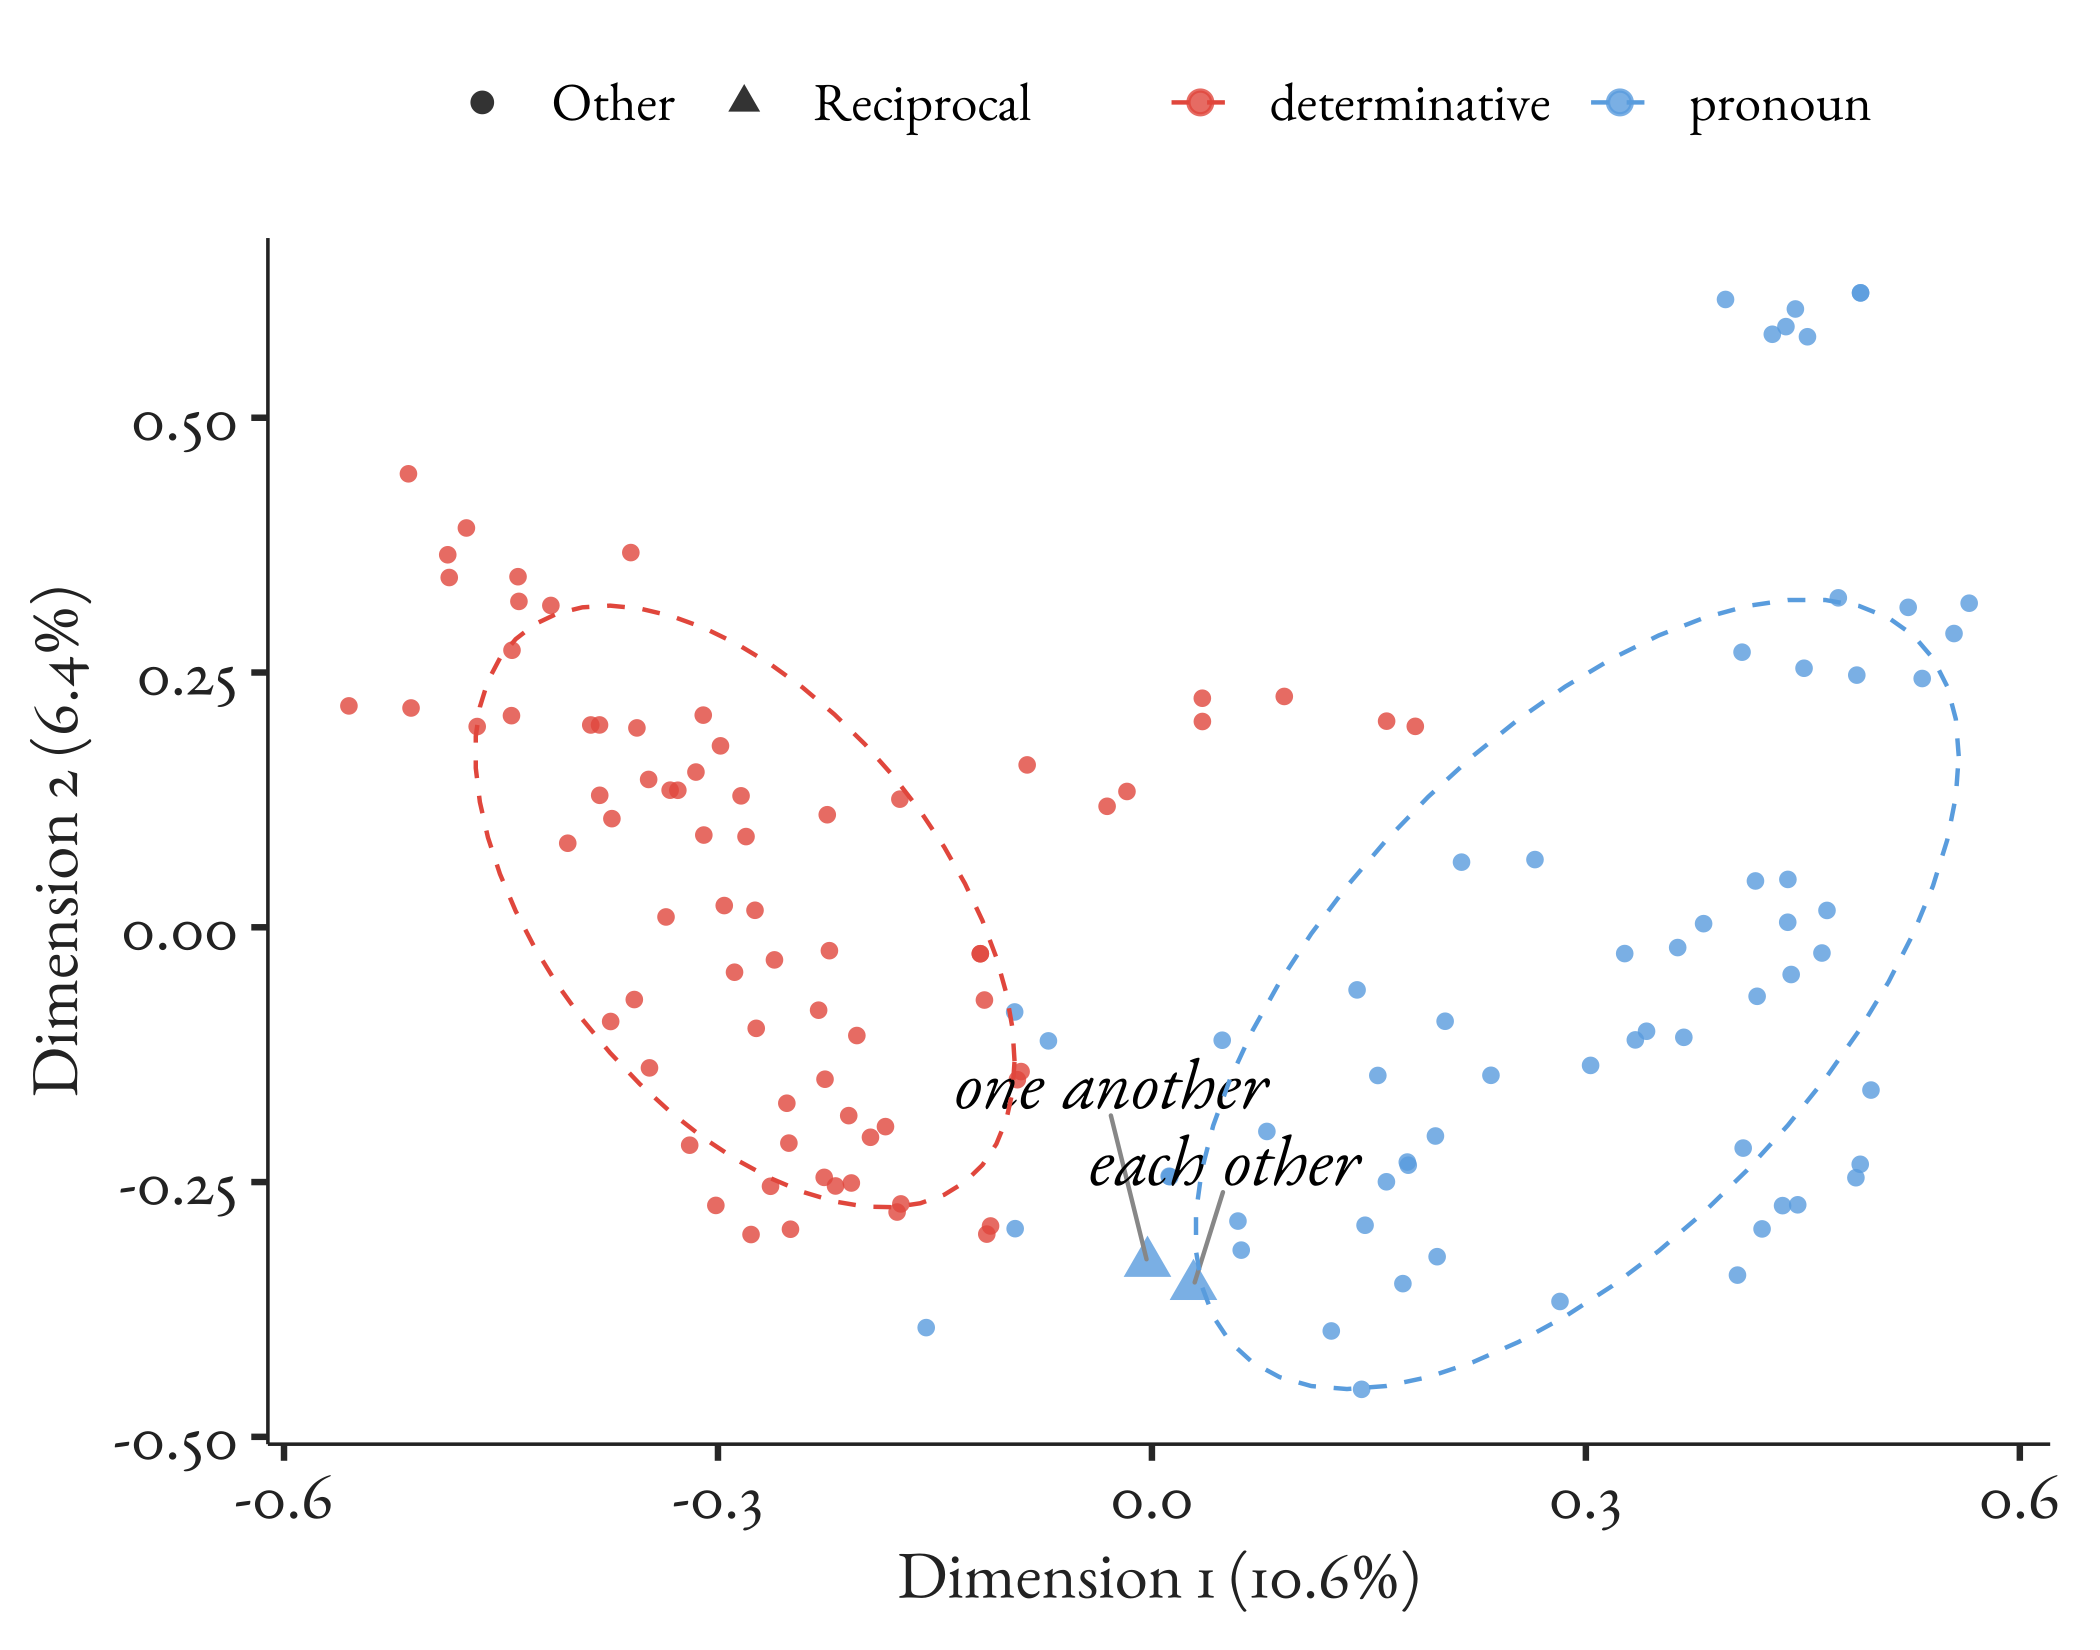
\includegraphics[width=\textwidth]{plots/mca_reciprocals.png}
    \caption{Reciprocals in grammatical feature space visualized with Multiple Correspondence Analysis. Pronouns (cyan) and determinatives (red) form regions; the compound determinatives sit at the interface; \mention{each other} and \mention{one another} (triangles) fall in that same interface.}
    \label{fig:mca}
\end{figure}

For comparison, I use two predeclared sets. First, canonical pronouns like \mention{he}, \mention{her}, and \mention{herself}. Second, the compound determinatives from \textcite[Ch. 5 \S9.6]{huddleston2002}, items like \mention{anybody} and \mention{everyone} that realize fused determiner-head functions \parencite{Payne2007}. If morphologically complex reciprocals pattern with anything, it is probably with these hybrids rather than with simple pronouns.

\begin{table}[!htbp]
    \centering
    \scriptsize
    \setlength{\tabcolsep}{4pt}
    \begin{tabular}{>{\raggedright\arraybackslash}p{0.16\textwidth} >{\raggedright\arraybackslash}p{0.19\textwidth} p{0.10\textwidth} p{0.12\textwidth} p{0.10\textwidth} p{0.13\textwidth}}
        \toprule
        Diagnostic & Illustration & Canonical pronouns & Compound determinatives & Reciprocals & Main pull \\
        \midrule
        Distinct case paradigm & \mention{he/him/his} & yes & no & no & determinative-ward \\
        Compound morphology & \mention{somebody}, \mention{each other} & no & yes & yes & determinative-ward \\
        Pronoun-like anaphoric NP substitution & standalone anaphoric NP use & yes & no & yes & pronoun-ward \\
        Fused determiner--head use & \mention{somebody arrived} & no & yes & no & pronoun-ward \\
        Reciprocal-style co-argument dependency & \mention{They liked each other} & no & no & yes & distinctive \\
        Subject distribution & \mention{He arrived}, \mention{Somebody arrived} & yes & yes & no & distinctive \\
        Reciprocal semantics & mutual interpretation & no & no & yes & distinctive \\
        Distinct pronominal genitive paradigm vs. clitic genitive & \mention{his}, \mention{somebody's}, \mention{each other's} & yes & no & mixed & mixed \\
        \bottomrule
    \end{tabular}
    \caption{Representative diagnostics encoded in the 155-property matrix. The full matrix contains many more items and finer distinctions; this subset shows the kinds of evidence that pull reciprocals toward pronouns, toward compound determinatives, or away from both.}
    \label{tab:diagnostics}
\end{table}

Table~\ref{tab:diagnostics} gives a compact view of the kinds of evidence that feed the matrix. The quantitative sections do not replace these diagnostics; they aggregate them, check their joint stability, and show how much the overall boundary reading depends on metric choice, feature family, and comparator choice.

From here the pipeline is straightforward. I first locate the reciprocals in the feature space, then summarize their relative position with a single distance contrast:
\[
\Delta = \bar d(\text{reciprocals},\text{pronouns})
       - \bar d(\text{reciprocals},\text{compound determinatives}).
\]
Positive values mean that reciprocals are closer to the compound determinatives than to the pronouns; negative values mean the reverse.

The later sections then ask four separate questions about that contrast: whether it is unusual under a constrained benchmark, how much it depends on numerical specifications, how much it depends on the chosen comparison groups, and what predictive blend best captures the reciprocals' position relative to clear anchors.

\FloatBarrier

\section{Benchmarking the Distance Contrast Against a Constrained Reference Distribution}

Before treating a positive \(\Delta\) as evidence of a determinative-ward pull, I need to know whether this feature matrix would often generate such a contrast even if the observed item--property pairings were scrambled. The benchmark should keep two basic facts intact: how many properties each word has and how many words each property applies to.

Each word in the dataset has a certain number of properties (e.g., \mention{each other} has 23), and each property applies to a certain number of words (e.g., \texttt{inflects for case} applies to 75). These totals reflect real facts about English: pronouns tend to have case distinctions, most words cannot be gradable, and so on. Any benchmark that ignored those totals would be too weak to be informative.

The relevant comparison keeps those totals while randomizing which specific words have which specific properties. Repeating that operation gives a reference distribution for \(\Delta\) under a benchmark where the instrument's marginal structure is intact but the observed grammatical pattern is scrambled. If the observed determinative-ward contrast is near the centre of this distribution, it is a routine by-product of the matrix's row and column totals. If it is in the tail, the contrast is unusual relative to that constrained benchmark.

The quasiswap algorithm \parencite{miklos2004randomization} generates exactly this kind of controlled randomization. It rearranges the feature matrix through thousands of small swaps, always preserving how many features each word has and how many words have each feature. In practical terms, the reference distribution asks whether the reciprocals end up closer to the compound determinatives than to the pronouns by more than this matrix structure alone would ordinarily produce. It does not show whether reciprocals are \enquote{really} intermediate. It asks the narrower model-checking question: whether the determinative-ward component of the reciprocal profile is unusual under the constrained randomization.

\begin{figure}[h!]
  \centering
  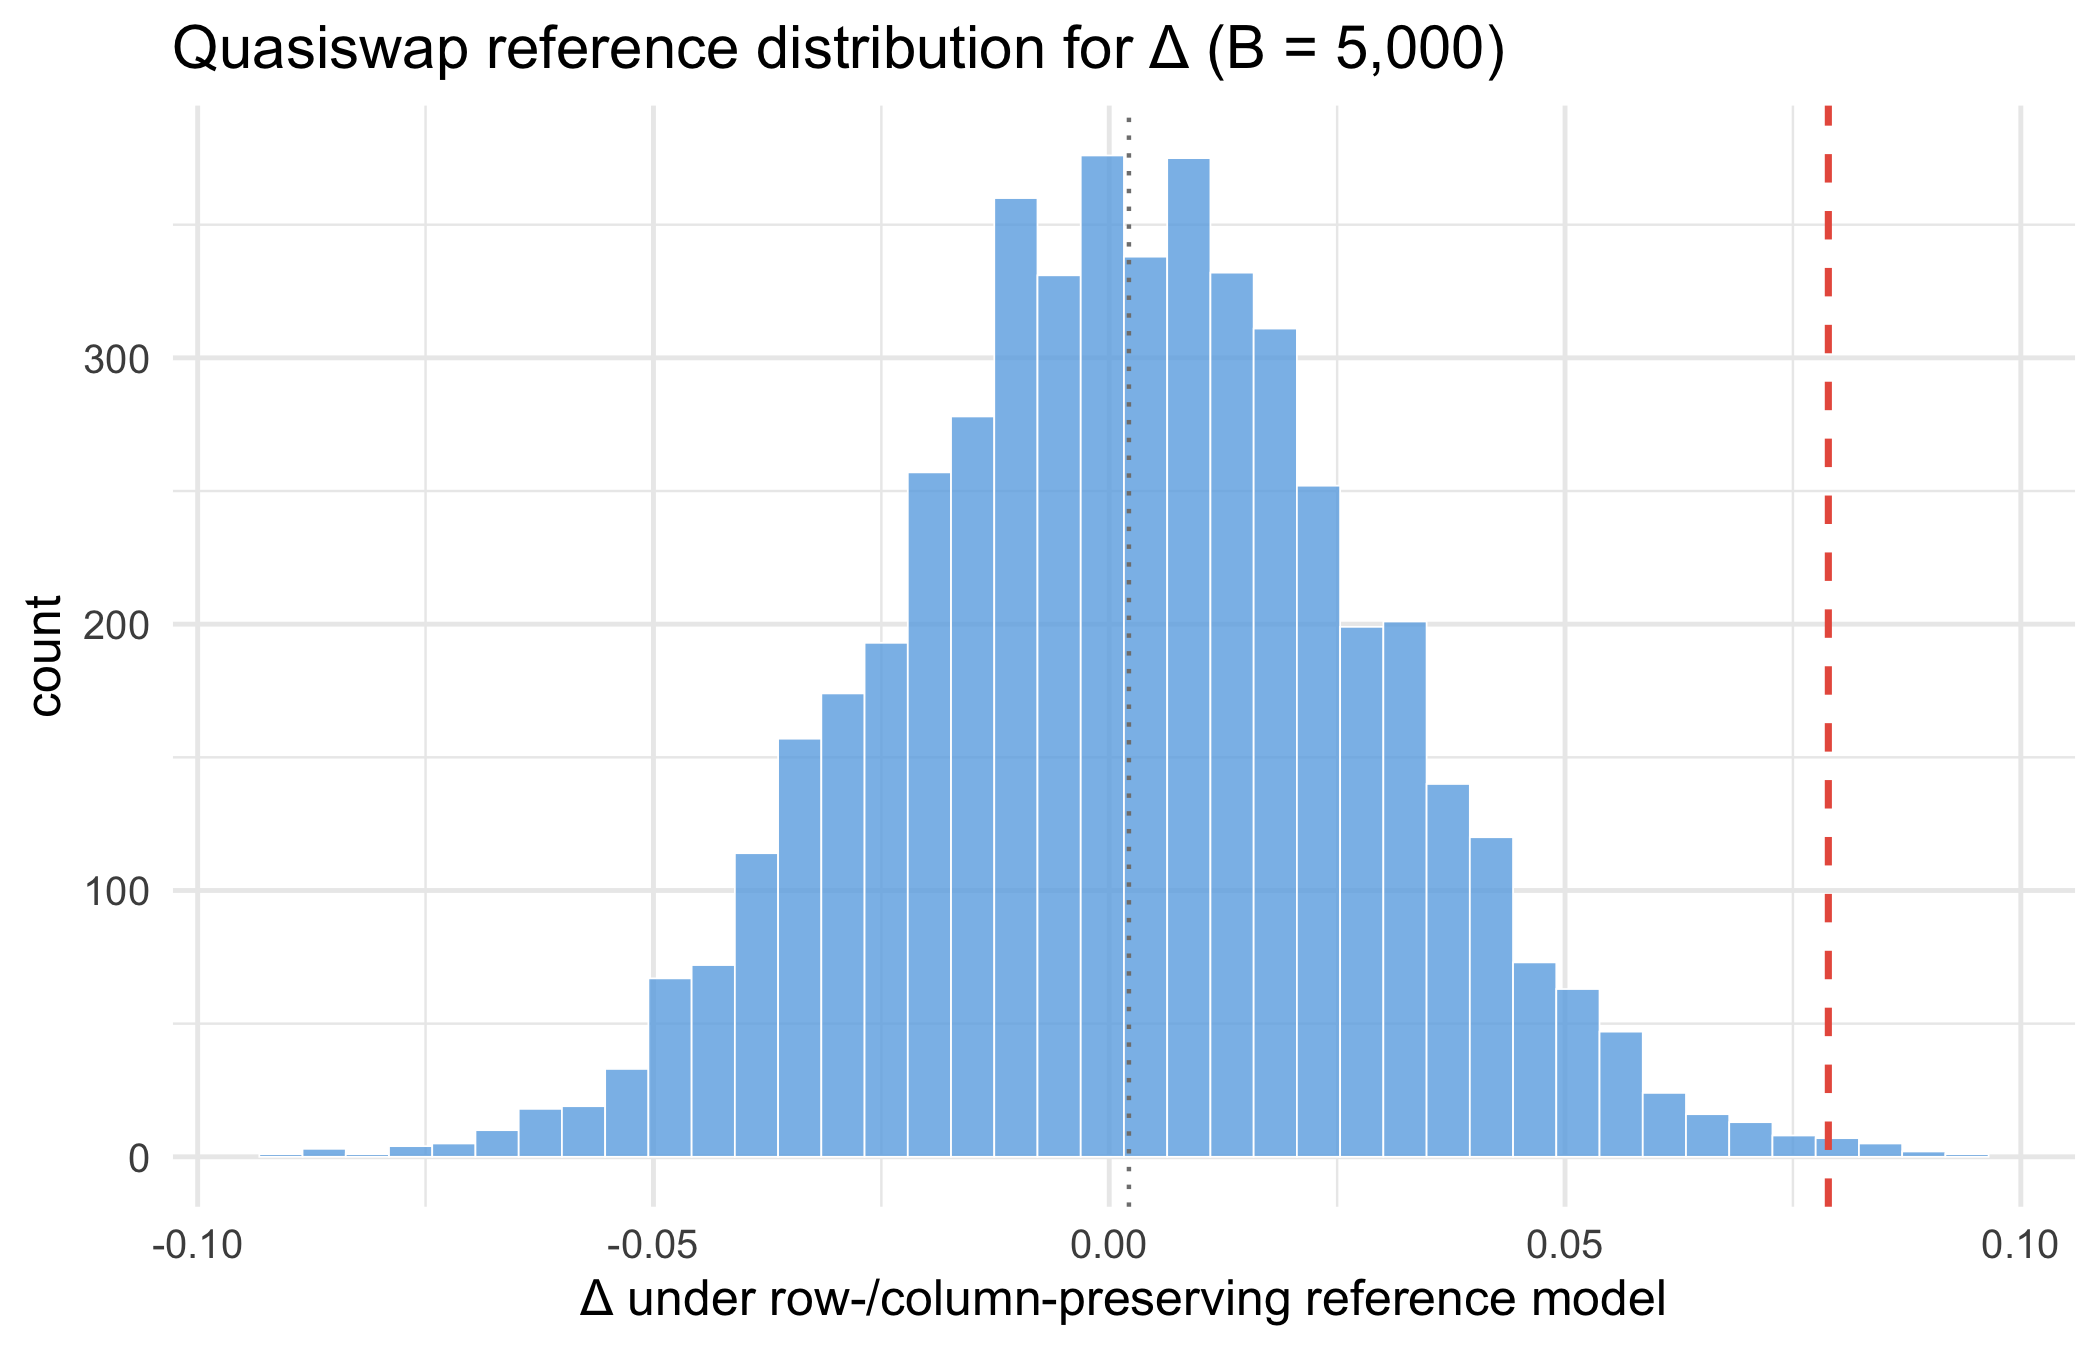
\includegraphics[width=0.72\textwidth]{plots/permutation_null.png}
  \caption{Constrained reference distribution for the observed \(\Delta\) contrast. The histogram shows \(\Delta\) values from 5,000 row- and column-preserving randomizations of the feature matrix, generated with the quasiswap algorithm; the dashed vertical line marks the observed value. The figure does not by itself establish boundary status. It shows that the observed determinative-ward contrast is unusual under this benchmark.}
  \label{fig:perm_test}
\end{figure}

The results are shown in Figure~\ref{fig:perm_test}. For my primary comparison, using carefully matched sets of six pronouns and six compound determinatives, the observed contrast falls in the extreme positive tail of this reference distribution (tail-area summary \(= 0.003\), Monte Carlo SE \(\approx 0.001\)).

I use this tail area as a model-checking summary, not as a classical test of a sharp null hypothesis. The reference model is intentionally artificial: it asks what \(\Delta\) values are typical when the instrument's row and column totals are preserved but the item--feature associations are otherwise scrambled. Under that benchmark, contrasts this determinative-ward are rare. That suggests the observed \(\Delta\) is not merely an artifact of how common or rare the coded features happen to be in English.

Two caveats apply. First, with only two reciprocals, no single contrast should carry much interpretive weight on its own. Second, my choice of which six pronouns and six determinatives to compare matters. Different selections might yield different results, a sensitivity I explore in section~\ref{sec:rotations}. For that reason, I treat the reference-distribution result as one model check on the determinative-ward contrast rather than as a decisive test of boundary status.\footnote{Implementation in \texttt{03\_matched\_set\_robustness.R}; reference draws saved as CSV/RDS for reproducibility.}


\section{The Garden of Forking Paths}

The reference-distribution check fixes one set of analysis choices: Jaccard as the primary distance, a specific set of reference items, and \(\Delta\) as the contrast of interest. Each choice is a fork in the path and an opportunity for bias to accumulate. The next question is whether the basic interface reading survives when reasonable alternatives are allowed.

Specification-curve analysis \parencite{simonsohn2020specification} addresses this directly. Instead of defending a single pipeline, I run many plausible pipelines and show all results. Here, I vary the distance metric (Jaccard, Dice, Hamming, and an IDF-weighted Jaccard), the feature set (all features, or blockwise ablations such as \enquote{no morphology} and \enquote{no syntax}), and the weighting method. The goal is not to find the \enquote{best} specification or crown a winning pipeline, but to see whether the sign and size of \(\Delta\) are stable across reasonable ones.

In the implementation, this regularization choice is parameterized by \(\alpha\); in Figure~\ref{fig:spec_curve} it is shown as the contrast between ridge and elastic-net weighting. The ridge method keeps all features in play with different weights, whereas elastic-net weighting allows the algorithm to drop weakly informative features altogether. Each combination yields a value of the same \(\Delta\), so the curve shows whether the contrast changes sign or merely changes size.

\begin{figure}[h!]
    \centering
    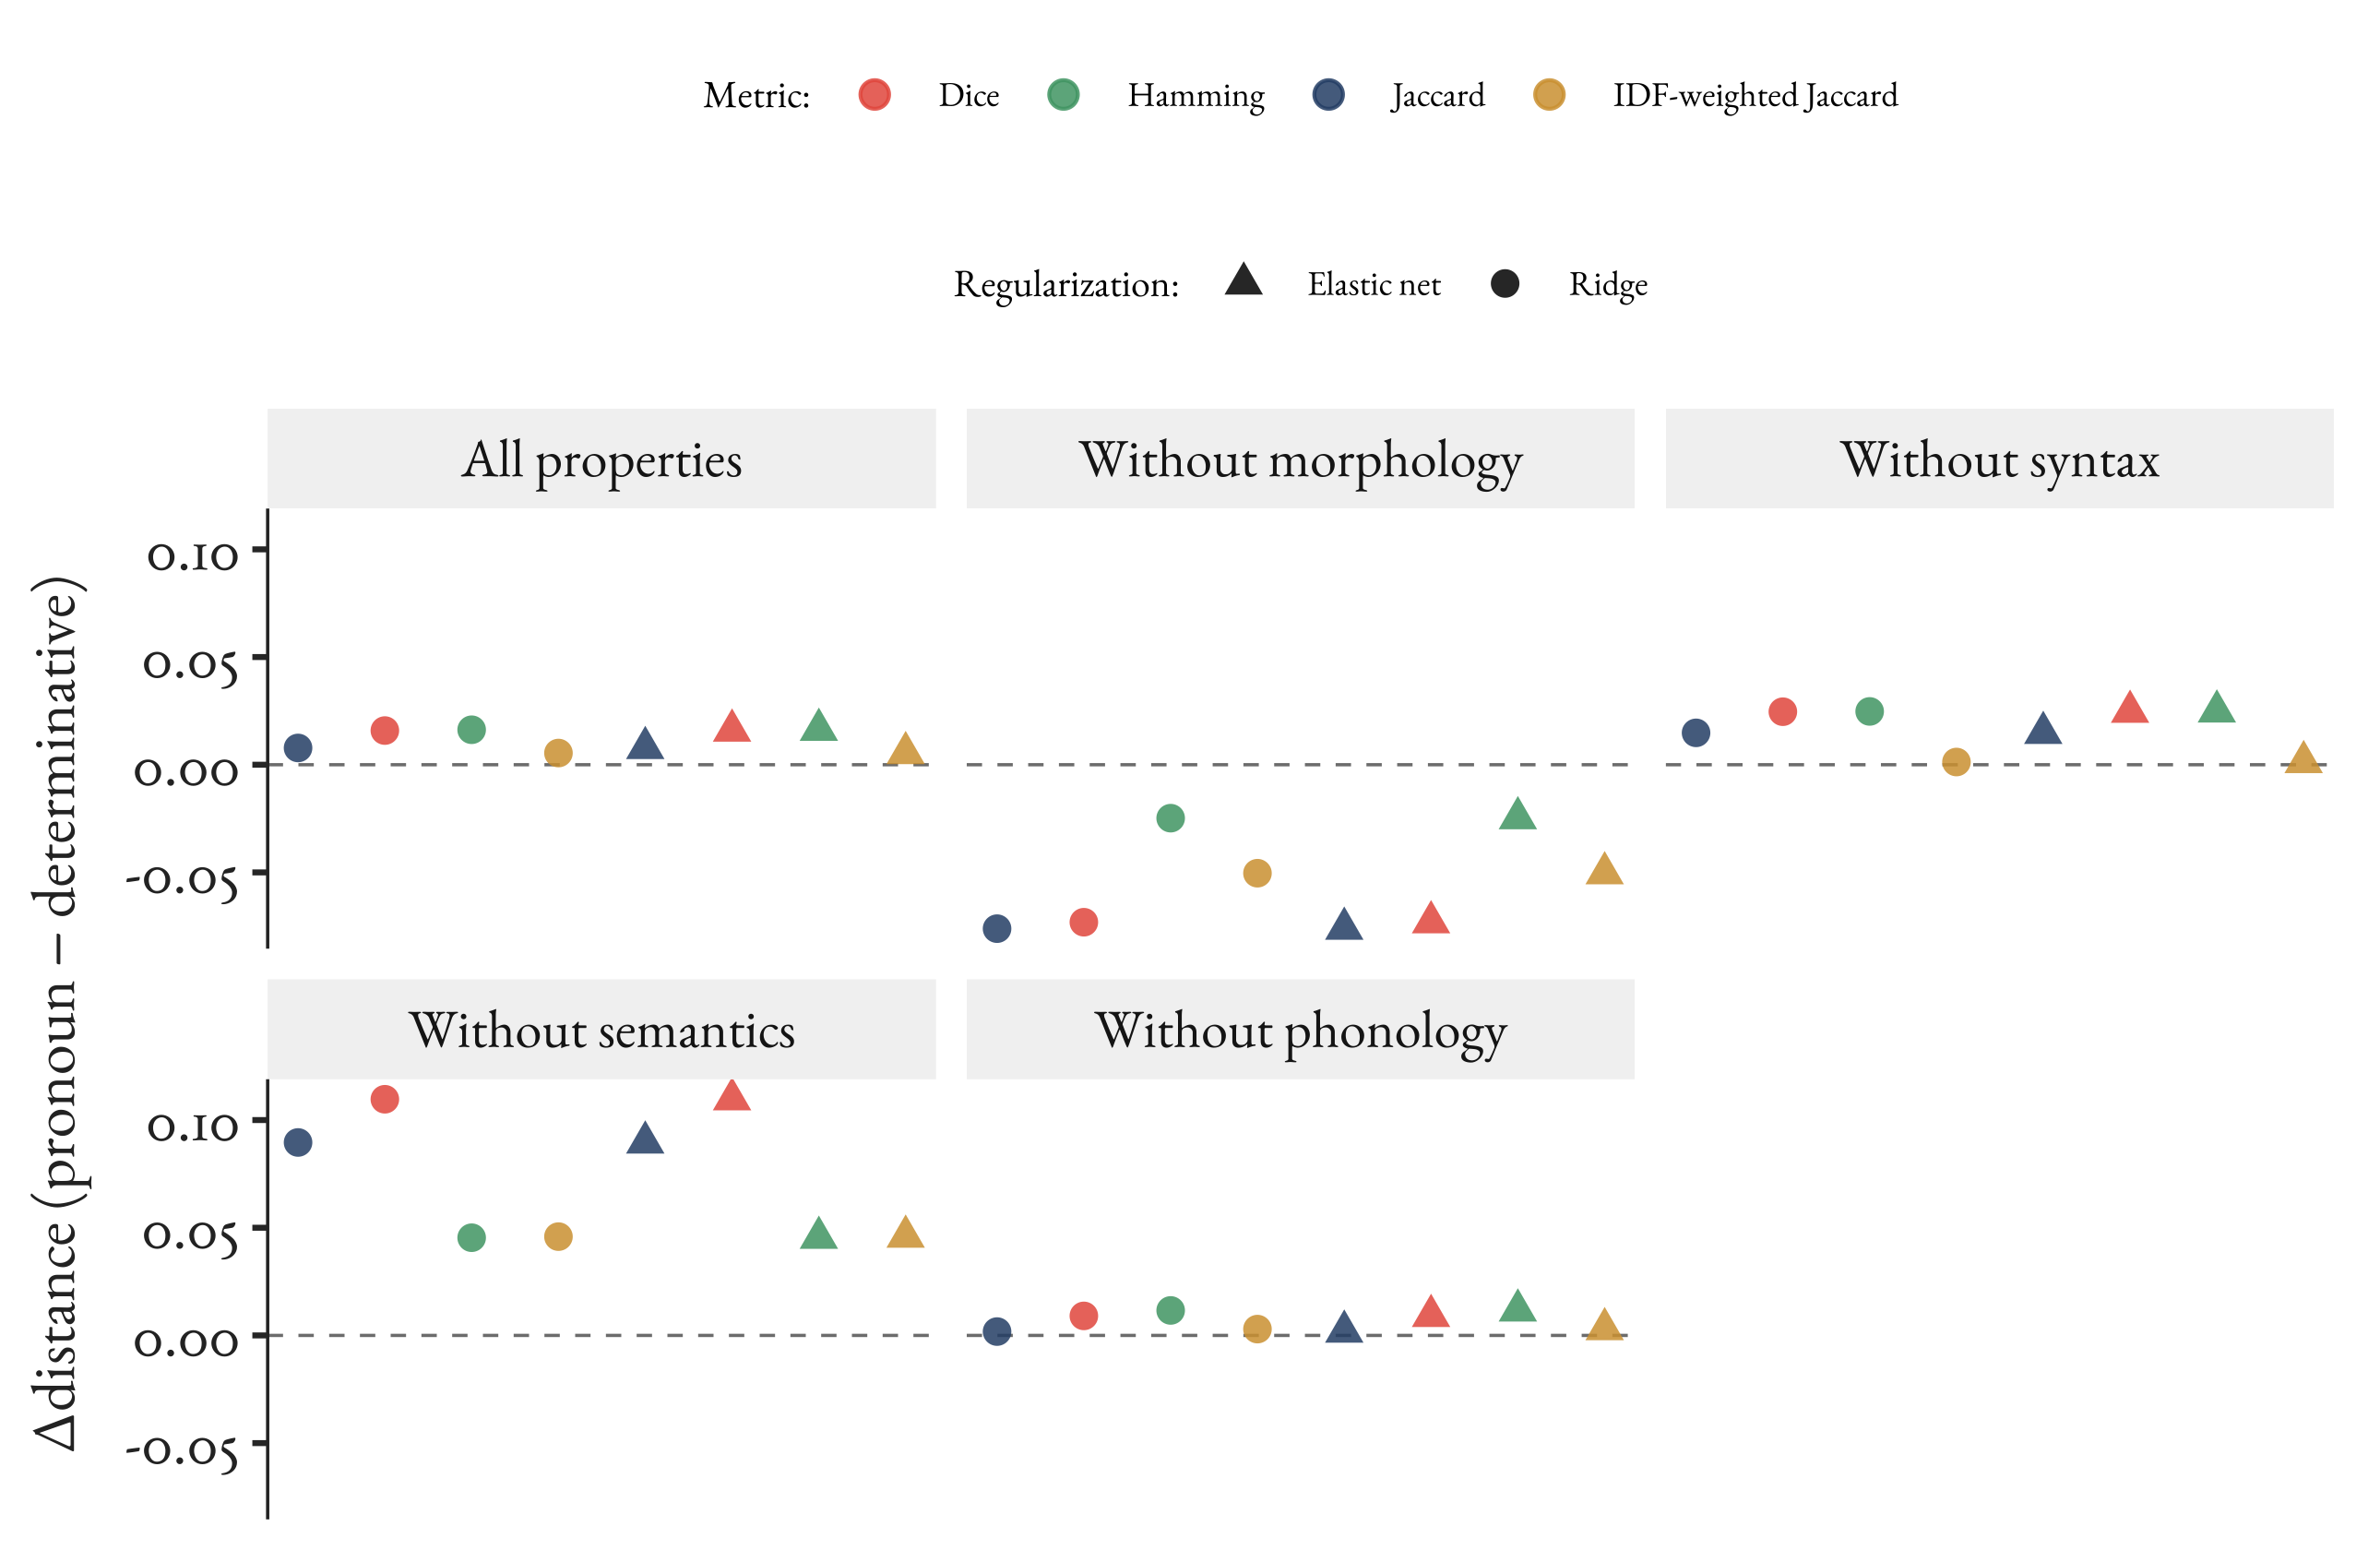
\includegraphics[width=\textwidth]{plots/spec_curve.png}
    \caption{Specification curve for $\Delta$. Each point shows the observed contrast under different combinations of weighting method (shape), distance metric (colour), and feature block exclusion (panels). Positive values indicate the reciprocals are closer to compound determinatives; negative values indicate they are closer to pronouns; zero marks the boundary.}
    \label{fig:spec_curve}
\end{figure}

Figure~\ref{fig:spec_curve} shows two clear patterns. First, the sign of \(\Delta\) is stable across distance metrics and weighting methods: most specifications land on the same side of zero. Second, only one block flips the sign. When morphology is \emph{excluded} (panel \enquote{morph}), \(\Delta<0\) and the reciprocals look more pronoun-like.

With all features included (panel \enquote{none}) \(\Delta>0\), and removing semantics pushes \(\Delta\) further positive (more determinative-like). Removing syntax or phonology leaves small, positive contrasts near the baseline. This pattern suggests that morphological features carry most of the determinative-ward signal, whereas semantic features contribute a pronoun-ward pull; syntax and phonology are comparatively weak in this contrast.

This invariance has theoretical significance. The specification curve does not settle any deeper ontology of categories on its own, but it does test whether the observed interface position is robust across reasonable metrics and ablations. $\Delta$ may shift in magnitude across specifications, but its sign, indicating which side of the pronoun/compound-determinative interface reciprocals favour, remains stable across most of them. Within this measurement model, that is the signature of a stable boundary position rather than a metric artifact.

What the specification curve does \emph{not} address is design sensitivity from the particular 6+6 matched sets used in the reference-distribution contrast; that is investigated separately by rotating the matched sets in section~\ref{sec:rotations}.

\section{The Importance of Comparison Groups}
\label{sec:rotations}

The specification curve addresses numerical tuning choices, but it keeps the comparator set fixed. The comparison-group question is different: how much depends on which anchor items I compare the reciprocals to? I had chosen specific pronouns and determinatives for comparison based on theoretical considerations, but different choices may yield different contrasts. To assess that design sensitivity, I repeated the analysis 100 times, each time randomly selecting six pronouns and six compound determinatives from the eligible pools while holding all other steps fixed.

\begin{figure}[h!]
    \centering
    
\includegraphics[width=0.8\textwidth]{plots/matched_subset_robustness.png}
    \caption{Sensitivity of $\Delta$ to the choice of comparison groups. The histogram shows the observed $\Delta$ values across 100 rotations of six pronoun and six compound determinative anchors. The dashed line marks the prespecified comparison set, the solid line marks the rotation median, and the dotted lines mark the interquartile range. Most rotations remain determinative-ward, but the magnitude varies substantially with the comparator set.}
    \label{fig:rotations}
\end{figure}

Figure~\ref{fig:rotations} shows wide variation across rotations.\footnote{Implementation: \path{03\_matched\_set\_robustness.R}; the specific canonical items are listed in \path{matched_subset_manifest.txt}.} The prespecified set yields \(\Delta = 0.079\); across rotations the median contrast is \(0.023\), with an interquartile range from \(0.002\) to \(0.043\). Three quarters of the rotations remain determinative-ward, but the effect is often much smaller than in the prespecified comparison.

With such small $n$, tail-area summaries are especially vulnerable to Type~S (sign) and Type~M (magnitude) errors \parencite{gelman2014types}, so the more informative summary is the distribution of $\Delta$ itself rather than a tail area attached to one matched set. The substantive point is that $\Delta$ is design-sensitive to the choice of comparators: the prespecified set sits high in the rotation distribution, but many equally reasonable comparator sets yield weaker contrasts.

Accordingly, I focus on the effect itself, the distance contrast \(\Delta\), and on how \(\Delta\) varies across rotations, using the rotations as a descriptive multiverse \parencite{steegen2016increasing} that quantifies uncertainty due to researcher degrees of freedom rather than as a filter for statistical significance.



\section{Predictive Calibration of Boundary Position}

The distance analyses ask which anchor set is nearer, but they do not give an intuitive scale for where the reciprocals sit between the two anchor profiles. To build that scale, I use a simple predictive blend model: a one-number summary asking what mix of pronoun-like and compound-determinative feature probabilities best predicts each reciprocal's observed profile.

The two category profiles are estimated from the anchor items with the reciprocals held out; the exercise asks how much of each profile best predicts a reciprocal's observed properties.\footnote{Concretely, the category profiles are fit on conservative clear-anchor sets. For each feature, the pronoun and compound-determinative anchor sets provide smoothed Bernoulli rates. For a given weight $w$, the blend probability is $w p_{\text{pron}} + (1-w) p_{\text{det}}$, and the predictive score for a reciprocal's 155-bit feature vector is its log loss under that blended profile. $\hat w$ is the minimizer. Implementation in \path{04\_weight\_calibration.R}.}

The model implements this idea with a mixture weight $w$ that ranges from 0 to 1. When $w = 1$, it predicts features from the pronoun profile; when $w = 0$, from the determinative profile. For values in between, it mixes the two patterns. At $w = 0.7$, for instance, it is 70\% pronoun-like and 30\% determinative-like. Read $w$ as a predictive index of boundary position, not as a literal claim about composition.

I then asked what mixture weight would make the model best match the reciprocals' observed feature patterns under the same scoring rule. In other words, if reciprocals are intermediate between the two anchor profiles, what blend best predicts their properties?

\begin{figure}[h!]
    \centering
    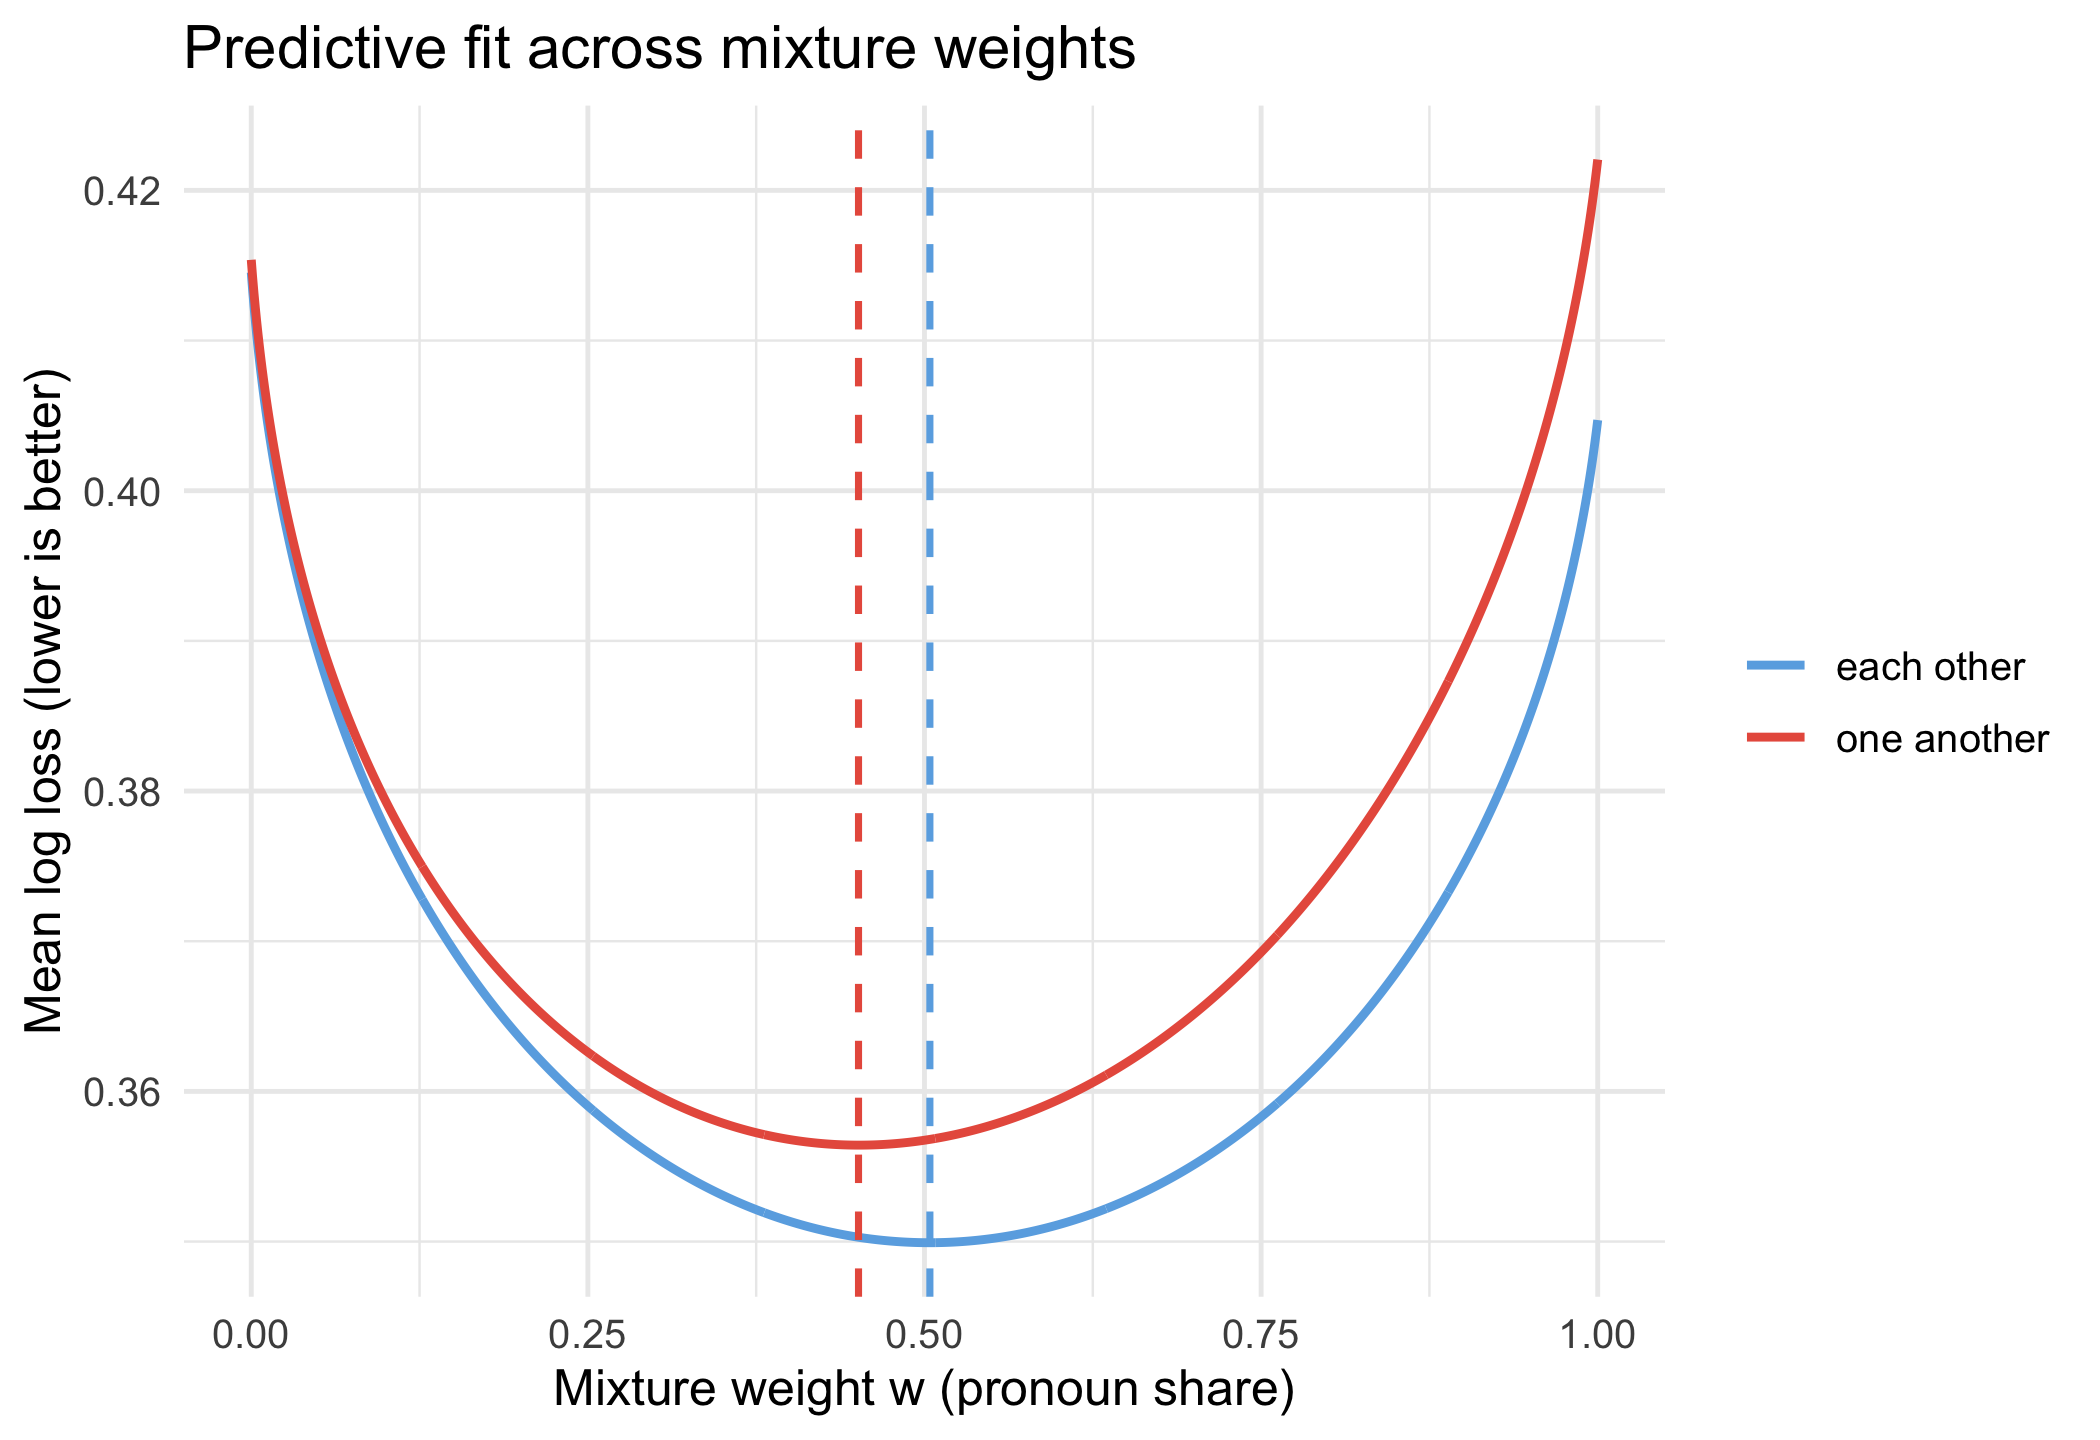
\includegraphics[width=0.8\textwidth]{plots/weight_calibration.png}
    \caption{Predictive blending of pronoun and compound determinative profiles. Curves show predictive fit as the mixture weight $w$ varies; dashed lines mark the best-fitting weights for each reciprocal. Both minima lie near parity, with $\hat w=0.504$ for \mention{each other} and $\hat w=0.451$ for \mention{one another}.}
    \label{fig:weight_cal}
\end{figure}

Figure~\ref{fig:weight_cal} reveals the same interface from another angle. To match the properties of \mention{each other}, the best blend is about 0.50 pronoun-like; for \mention{one another}, about 0.45 pronoun-like.

This provides another lens on the same phenomenon. Whether the analysis visualizes grammatical space, measures distances, compares the observed contrast to a constrained reference distribution, or calibrates this simple blend, reciprocals consistently appear at the interface rather than clustering near either anchor profile.

Two caveats apply. First, reciprocals are not literally probability mixtures of two kinds; the model provides an interpretable, one-number summary of where they sit relative to the anchor profiles. Second, the blend is estimated on the same measurement instrument as the other analyses, so it is another internal check rather than an independent source of evidence.


\section{Checking the Instruments}

Throughout these analyses, I have treated the feature matrix as a measurement model. The next issue is whether the measurements themselves are problematic. The first question is not whether the richest model fits, but whether the workflow earns trust step by step by distinguishing clear anchors and preserving basic structure before it is asked to interpret a case with unresolved placement. In other words, before asking the instrument to place the reciprocals, I need to know whether it can recover the easy cases.

The checks reported here start one step later. I fit a simple model that predicts each binary feature from the item's category label with modest adjustment terms and weak regularization, then draw replicated datasets from the fitted model.\footnote{Concretely, for feature $j$ on item $i$, $y_{ij}\sim\mathrm{Bernoulli}(\pi_{ij})$ with $\mathrm{logit}\,\pi_{ij}=\alpha_j+\beta_j\mathbf{1}\{c_i=\text{pronoun}\}$ and ridge regularization on $\beta_j$; draws are parametric bootstrap replicates (posterior draws if a Bayesian fit is used). Reciprocals are held out wherever predictions for them are reported.} That staged buildup matters because a complicated fit can look plausible while still hiding an implementation error.

I ask two related questions: whether replicated datasets preserve the large-scale arrangement under the same ordination, and whether they preserve nearest-neighbour relations around anchors.

\begin{figure}[h!]
    \centering
    \begin{subfigure}[b]{0.46\textwidth}
        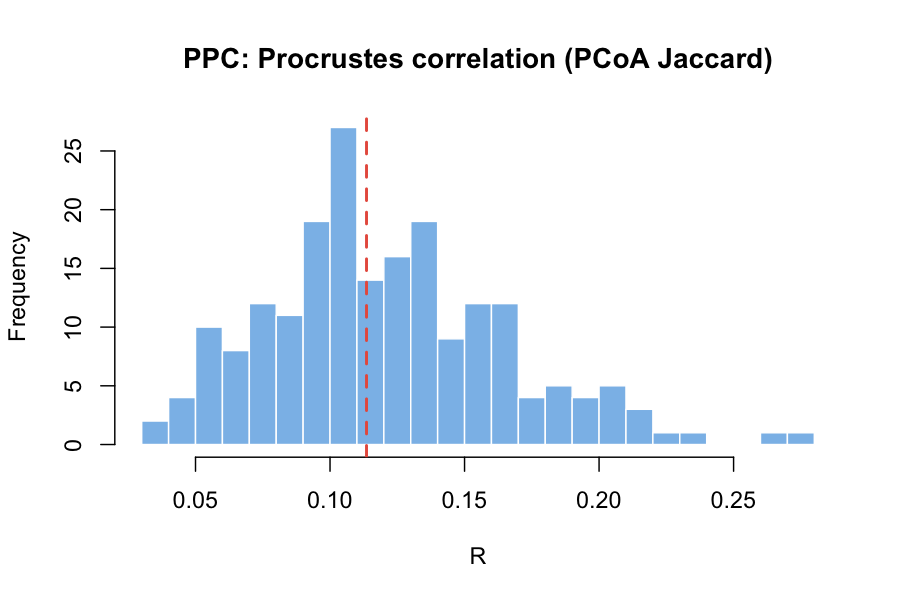
\includegraphics[width=\textwidth]{plots/ppc_procrustes_hist.png}
        \caption{Predictive check for global structure. Histogram: distribution of the Procrustes statistic under replicated datasets; vertical line: observed statistic.}
        \label{fig:ppc_procrustes}
    \end{subfigure}
    \hfill
    \begin{subfigure}[b]{0.46\textwidth}
        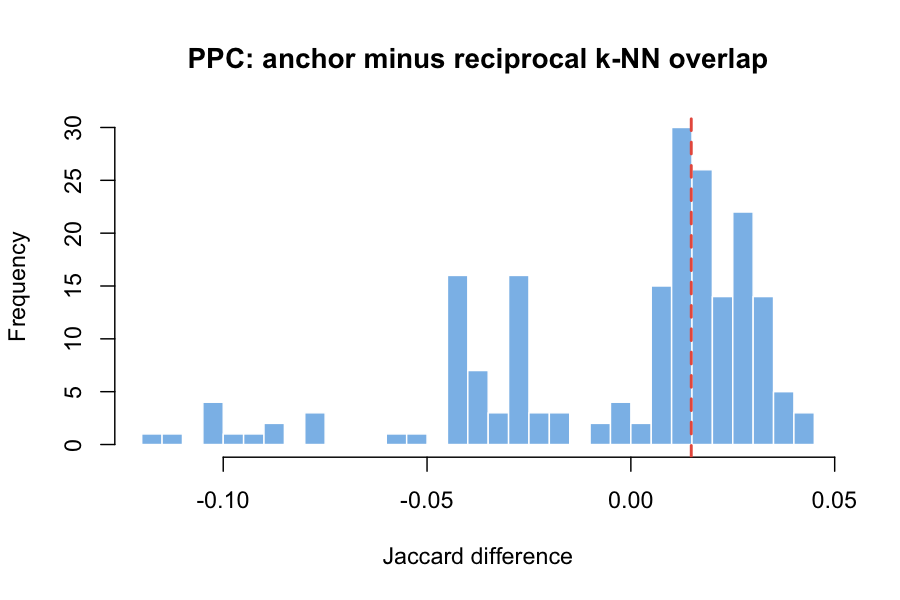
\includegraphics[width=\textwidth]{plots/ppc_knn_diff_hist.png}
        \caption{Predictive check for local structure. Histogram: distribution of $k$-NN overlap around anchors ($k$ fixed across runs); vertical line: observed overlap.}
        \label{fig:ppc_knn}
    \end{subfigure}
    \caption{Predictive checks. (a) Global structure: distribution of Procrustes fit statistics across replicated datasets (histogram) with the observed statistic marked (vertical line). (b) Local structure: distribution of nearest-neighbour overlaps under replication, with the observed overlap marked.}
\end{figure}

%different colour may be more visible

\begin{figure}[h!]
    \centering
    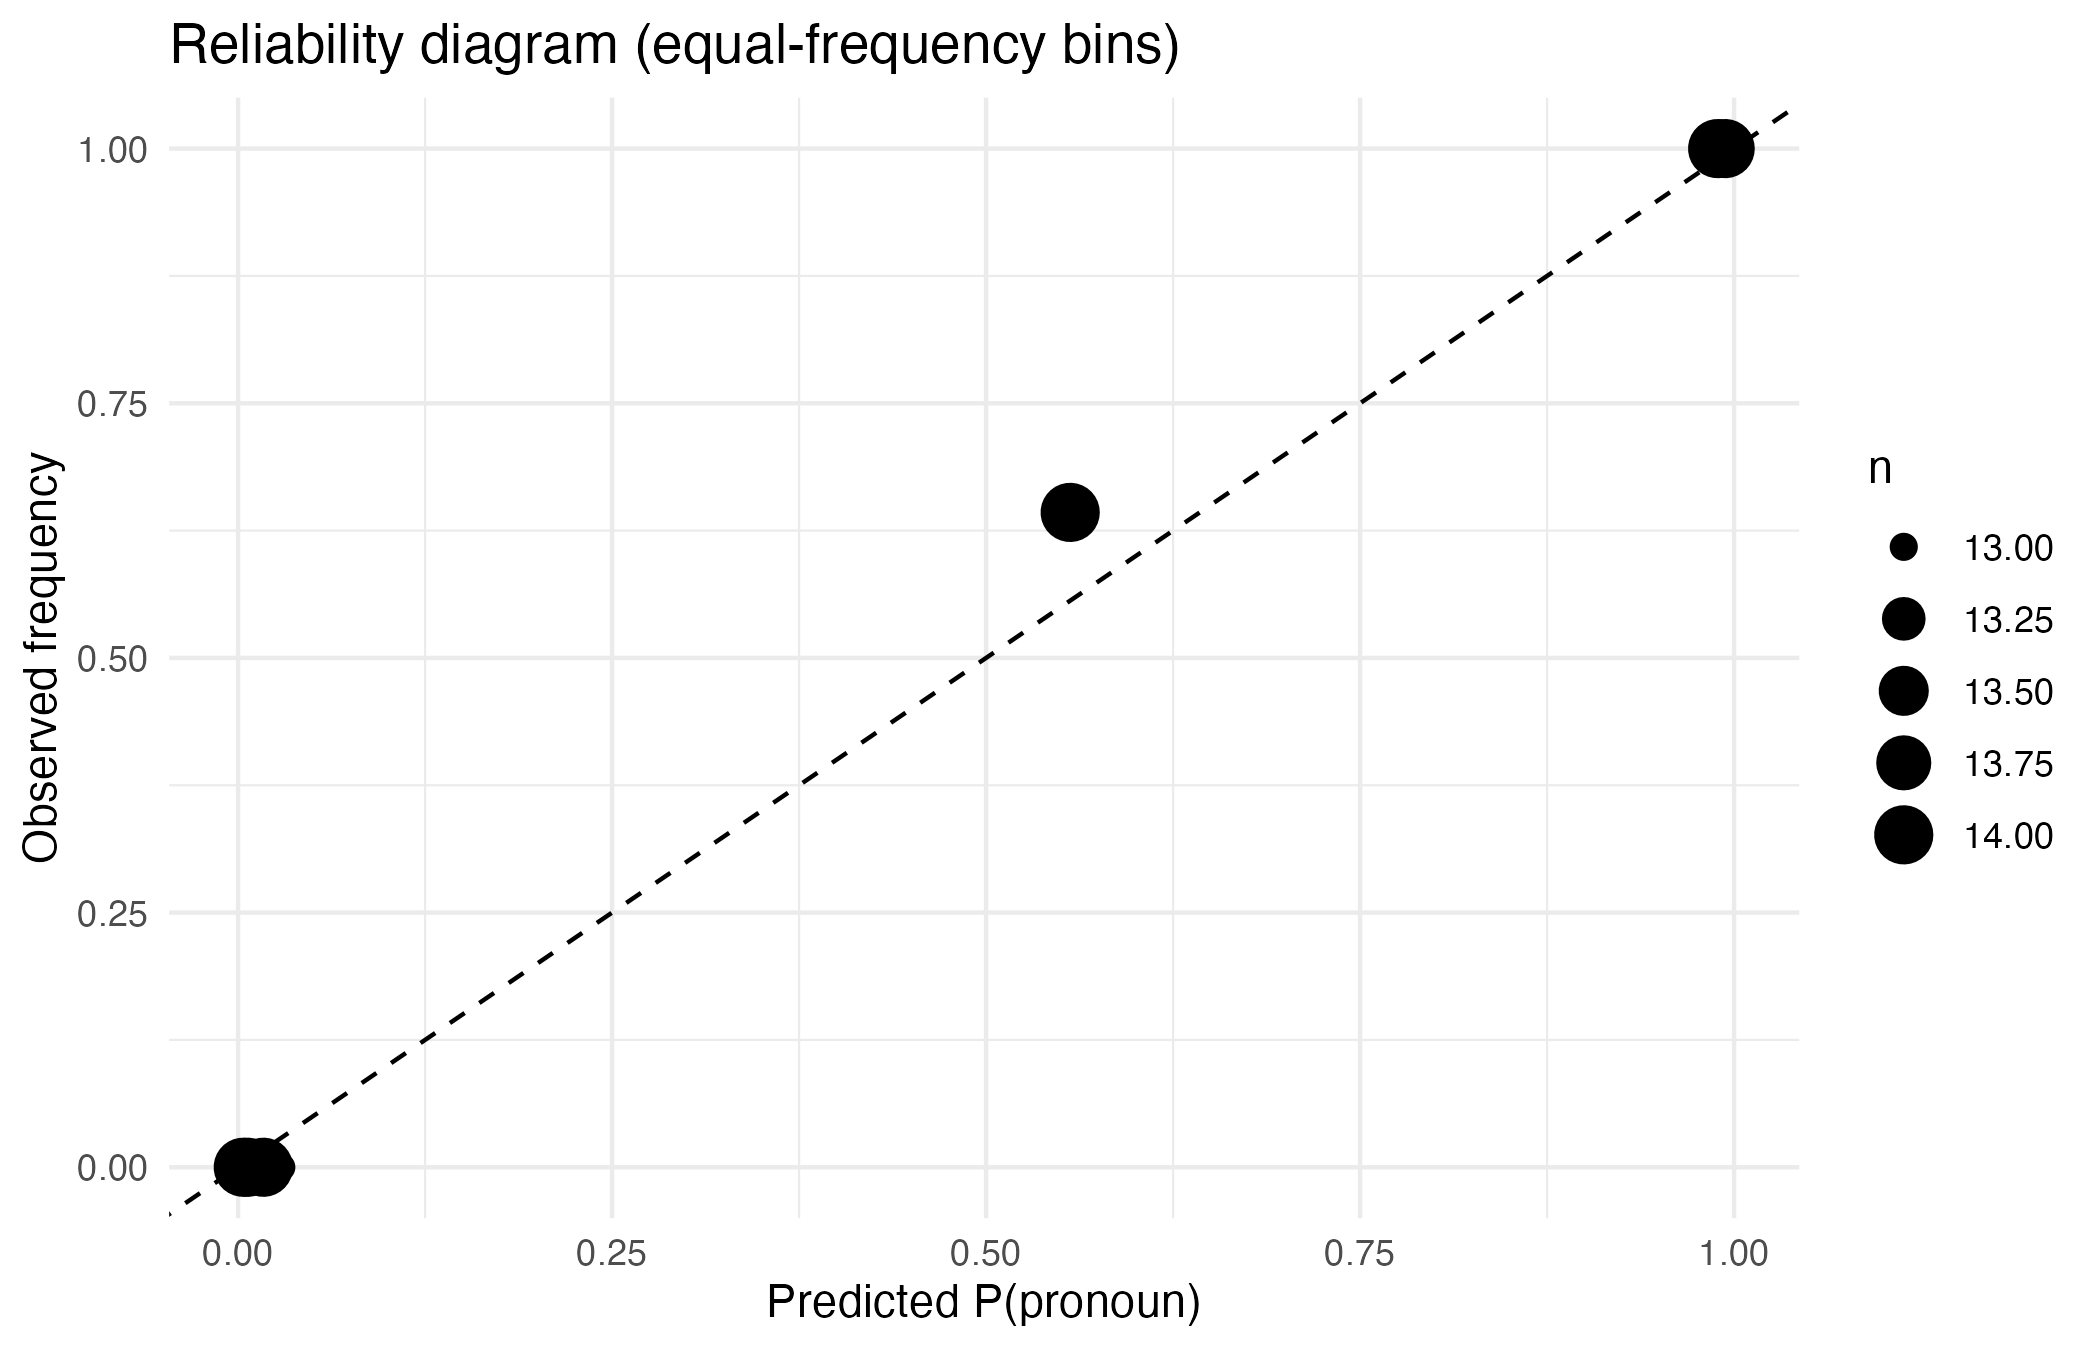
\includegraphics[width=0.7\textwidth]{plots/calibration.png}
    \caption{Reliability diagram under cross-validation, following \textcite{niculescu2005predicting}. Predicted probabilities (x-axis) track observed frequencies (y-axis), showing approximate calibration: when the model predicts 70\% probability for the pronoun label, about 70\% of held-out items are pronouns.}
    \label{fig:calibration}
\end{figure}

The model passes these basic predictive checks (Figures~\ref{fig:ppc_procrustes}, \ref{fig:ppc_knn}, and~\ref{fig:calibration}). Replicates maintain reasonable global geometry and preserve about 65.5\% of local neighbourhood structure around anchors. The reliability diagram shows that when the classifier assigns, say, 70\% probability to the pronoun label, the realized frequency on held-out items is near that level, so probabilities are roughly calibrated rather than systematically over- or under-confident.\footnote{For the reciprocals, the classifier assigns near-chance pronoun probabilities (0.485 for \mention{each other}, 0.467 for \mention{one another}); masked predictive log-likelihood is identical under either labelling ($-54.240$), and per-item cross-entropy is $0.371$ versus a chance baseline $\ln 2 \approx 0.693$.}

Perfect reproduction is neither expected nor desired. What matters is that the measurement model carries real signal about categorical structure: clear pronouns and clear compound determinatives are distinguishable under the same machinery, which makes the reciprocals' unresolved placement informative rather than an artefact of a broken instrument.



\section{Results for Grammatical Boundaries}

These results match the projectibility claim introduced above. If the reciprocals occupy a stable boundary position, their placement should survive reasonable changes in metric and feature set, different feature blocks should pull in different directions, clear anchors should remain recoverable, and a predictive blend should place the reciprocals near parity. That is the pattern observed here: the sign of the distance contrast is stable across metrics and penalties and is only modest in magnitude, while reference-distribution extremity is design-sensitive even though the qualitative boundary diagnosis persists across rotations.

The blockwise results supply the expected cross-dimensional tension: morphology contributes most of the determinative-ward pull while semantics contributes a pronoun-ward pull, with syntax and phonology comparatively weak in this contrast. The instrument also separates anchors and yields calibrated supervised probabilities for them. The predictive blend places both reciprocals near parity, and the prespecified anchor contrast sits in the extreme tail of the row- and column-preserving reference distribution even though its extremity is design-sensitive across rotations.

This pattern is compatible with the homeostatic property-cluster view of categories. The reciprocals exhibit stable interface placement with cross-dimensional tension rather than a decisive recategorization or a failure of measurement. Within this instrument, no cutoff, classifier, or blend model can make morphology and semantics agree when they do not; changing the conclusion would require different measurements or external evidence, not a different threshold.

More generally, boundary items should be expected to show stable interface placement under reasonable analytic choices. Single diagnostics or cherry-picked features force binary decisions; comprehensive profiles, prespecified lenses, and summaries that propagate design uncertainty instead map the topology of grammatical space, including its interfaces, and make clear what is robust within the chosen measurement model.


\section{Discussion}

On an HPC view, success at a boundary is not a decisive recategorization but a stable pattern of diagnostic uncertainty accompanied by cross-dimensional conflict. That is the profile reciprocals exhibit here. Across lenses that make different invariance assumptions but interrogate the same measurements, reciprocals sit at the edge of the pronoun region in ordinations, show mixed nearest neighbours, attract near-chance supervised probabilities with tied predictive fit (0.485, 0.467; log-likelihood $-54.240$ under either labelling), and display a blockwise split in which morphology leans determinative-ward,\footnote{This likely reflects pronouns' tendency to inflect for case, which reciprocals resist.} semantics leans pronoun-ward, and syntax and phonology contribute relatively little.

Read through the HPC lens, the mixture calibration reproduces decisive separation for anchors while placing reciprocals at the boundary with near-parity placement, consistent with the ordination, distance, reference-distribution, and supervised results. Because all lenses interrogate the same measurements, agreement is internal robustness rather than independent convergence.

The blockwise pattern is compatible with a cautious HPC interpretation, but it does not identify the mechanisms themselves. The relevant idea is simple: if a category is held together by several partly independent systems, different parts of its feature profile can be stabilized in different ways. For reciprocals, morphological realization rules and agreement systems could support the morphology-ward pull, while interpretive mechanisms governing reference tracking, binding, and argument structure could support the semantics-ward pull. The measurements do not show those systems directly. They show the cross-dimensional tension that this kind of category model predicts. The paper's direct claim remains measurement-level rather than metaphysical: in this \textit{CGEL}-informed feature space, reciprocals occupy a stable position at the pronoun/compound-determinative interface.

What the instruments reveal is proximity to that interface: near-chance classifier probabilities, near-parity mixture weights, and cross-dimensional tension. The situation is analogous to a microscope at its resolution limit. The instrument localizes an interface zone even when it does not settle every deeper question about underlying ontology, and the 155-feature matrix has an analogous resolution floor within which the reciprocals fall. That uncertainty is epistemic rather than ontological: the measurements place reciprocals in an interface zone, but they do not show that the underlying categories themselves are vague or graded.

This interpretation also clarifies what the results do not show. The analyses do not accumulate independent evidential weight; all procedures reuse the same hand-coded matrix. Agreement across lenses counts as internal robustness against method-specific artifacts rather than as independent convergence, and the numbers do not by themselves license recategorization. On the predeclared matched set the observed contrast sits far into the positive tail of the row- and column-preserving reference distribution (tail-area summary \(= 0.003\)), but across rotated comparison sets the effect size varies substantially. Under an HPC reading, that combination of modest directionality, design sensitivity, and stable qualitative diagnosis is what an interface position should look like given a target population of only two types.

The fusion-of-functions architecture provides a complementary grammatical backdrop \parencite{Payne2007}. If category and function are distinct primitives and fused determiner--head structures are grammatically real, then these morphologically complex items can be determinatives by category while serving fused determiner--heads in NP. That architecture predicts pressure toward categorical edges when different mechanisms sustain partially conflicting property bundles. The measurements above are consistent with such pressure for the reciprocals: they behave pronoun-like on some property clusters and determinative-like on others. At the same time, retaining the canonical \textit{CGEL} pronoun analysis as the prior default is methodologically appropriate; the data here do not overturn it, and the framework shown here makes explicit what kinds of evidence would do so.

Seen more broadly, the study's contribution is methodological and interpretive rather than a category assignment. It operationalizes a way to examine boundary phenomena that avoids selective diagnostic shopping \parencite{croft2001radical}: prespecify a small set of sensible lenses; interpret agreement as internal robustness on one dataset; make prior theoretical commitments explicit; and report the full specification surface rather than only favourable summaries. Inconclusive tests cease to be mere failures when they co-occur with cross-dimensional conflict and a stable pattern of diagnostic uncertainty; they become data about the structure of categories if those categories are homeostatic clusters \parencite{miller2021}.

\subsection{Limitations, scope conditions, and disconfirmation}

All findings are conditional on a single, theory-informed, hand-coded binary measurement model. Features are binarized, single-coder, and \textit{CGEL}-dependent; this raises construct-validity and reliability concerns. I partly offset these with blockwise analyses and metric choice motivated by ordination, but stronger guarantees would require multi-annotator coding with reliability estimates or corpus-derived distributional features that reduce theory-dependence.

Target scarcity constrains inferential resolution: English has two reciprocal types, so any single reference-distribution contrast between reciprocals and comparators is inherently fragile, and supervised categorization produces only two probabilities of primary interest. Multiplicity and researcher degrees of freedom are addressed by prespecifying a small, theory-led set of lenses and reporting all analyses. Specification choices nonetheless remain scope conditions on the results.

External validity is restricted to English and to the inventory defined by \textit{CGEL}; cross-linguistic generalization is a matter for new data.

The framework also supplies clear disconfirmation criteria for this case. Outcomes that would count against the boundary diagnosis include: alignment of morphology, syntax, semantics, and phonology on the same pole; calibrated supervised probabilities near 1.0 under one labelling together with superior predictive fit; disappearance of diagnostic uncertainty under reasonable distance metrics or regularization choices; and stability of those outcomes under feature-subset resampling. None of these criteria is met here.

\subsection{Implications and outlook}

This case illustrates how to study boundary phenomena responsibly when categories are treated as homeostatic clusters. The objective is not to force a verdict on reciprocals but to refine the workflow that registers boundary behaviour on the measurement model already in use.

The first implication is that the workflow should characterize dependence rather than \enquote{repair} individual codings in a large, noisy matrix. What matters is which parts of the measurement model underwrite the boundary diagnosis. Influence diagnostics for distance-based summaries, blockwise ablations, and adversarial recoding of plausible high-leverage features can map an internal robustness surface: they show which modest, theory-motivated perturbations do and do not alter the qualitative outcome. Predictive comparison belongs in this workflow only after posterior predictive checks and with Pareto-$k$ diagnostics reported, since its role here is secondary to the main question of boundary location rather than model ranking.

The second implication is calibration against control items. Clear pronouns and clear compound determinatives should behave as anchors under the same lenses, yielding high-confidence, aligned outcomes for anchors and diagnostic uncertainty for reciprocals. If the same uncertainty appears for anchors, the pipeline is uninformative; if it localizes to reciprocals, the boundary reading gains credibility without appealing to data beyond the current inventory. An anonymized supplement accompanying this submission provides the full matrix, feature-block map, item annotations, anchor manifests, scripts, matched-set manifest, quasiswap draws, and derived robustness summaries so that readers can inspect which coding decisions do and do not move the interface position.

A third implication concerns evidence beyond the type-level matrix. Token-level evidence, where available, should be used as a diagnostic of boundary dispersion rather than as a route to a type-level decision. The lexeme can be treated as a distribution over constructions and modification profiles, with predeclared dispersion summaries compared to the anchors. Under a cluster view, a boundary item is expected to show broader, more heterogeneous contextual support than clear-category anchors. Independent acceptability judgments offer a complementary test: if distance-to-boundary predicts judgment variance in contexts that differentiate pronouns from determinatives, that would support the interpretation that stable diagnostic uncertainty reflects proximity to a discrete threshold rather than inherent category fuzziness.

These implications remain within English and within the existing theoretical commitments, but the logic transfers. Field linguists documenting boundary phenomena in understudied languages may not need elaborate statistical machinery at the first stage. The core practice is still portable: document the full range of conflicting properties, compare explicitly to clear anchors, and acknowledge boundary status in reference materials rather than forcing binary decisions. That is the broader payoff of the workflow: it makes difficult category edges inspectable without pretending that every hard case can be made decisive.


\section{Conclusion}

Boundary phenomena in grammatical categorization need methods that can distinguish unstable coding noise from stable interface placement, especially when the target inventory is small. The analysis above offers such a method for English reciprocals. Starting from a 155-property \textit{CGEL}-informed profile of pronouns and determinatives, it asks whether \mention{each other} and \mention{one another} keep returning to the same region of grammatical space under randomized benchmarks, alternative specifications, rotated comparison sets, predictive blending, and anchor calibration.

The answer is yes, but it is not a binary recategorization. Across the lenses applied above, reciprocals occupy the pronoun/compound-determinative interface. They show mixed neighbours, stable distance contrasts, near-parity blend weights, and calibrated uncertainty in supervised models, while morphology pulls them toward compound determinatives and semantics pulls them toward pronouns. This stability is informative because it is not the pattern expected from arbitrary coding noise or an uninformative pipeline: clear anchors remain recoverable, and the same diagnostics localize uncertainty to the difficult items. At the same time, the evidence is internal robustness on one hand-coded measurement model, not independent convergence across datasets. The uncertainty is epistemic; the measurements locate an interface zone without showing that the underlying categories are themselves vague.

That measurement-level result can be read through an HPC account without depending on that account for its basic force. On a homeostatic property-cluster view, categories are useful because partially observed profiles support projections to further properties. Clear pronouns and clear compound determinatives do that here; the reciprocals are revealing precisely because those projections conflict in stable, structured ways. The result therefore does not overturn the standard pronoun treatment in \textit{CGEL} or prove that reciprocals form a separate category. It gives a narrower characterization: within this feature space, they occupy a stable peripheral position in the pronoun system at the boundary with determinatives.

The broader payoff is methodological. For small-$n$ boundary cases, the task is to make the specification surface inspectable: build comprehensive property profiles, show representative diagnostics, use ordination to guide distance summaries, compare key contrasts to constrained reference distributions, vary reasonable specifications, calibrate against clear anchors, and report effect distributions rather than only tail areas. Those steps will not make hard cases easy, and they should not be treated as a substitute for new measurements or external evidence. They make hard cases harder to misdescribe.


\clearpage
{\centering\textsc{References}}

\begin{sloppypar}
\printbibliography[heading=none]
\end{sloppypar}

\end{document}
